\documentclass[aspectratio=169,notes]{beamer}
% \documentclass[aspectratio=169]{beamer}
\usetheme[faculty=phil]{fibeamer}
\usepackage{polyglossia}
\setmainlanguage{english} %% main locale instead of `english`, you
%% can typeset the presentation in either Czech or Slovak,
%% respectively.
\setotherlanguages{russian} %% The additional keys allow
%%
%%   \begin{otherlanguage}{czech}   ... \end{otherlanguage}
%%   \begin{otherlanguage}{slovak}  ... \end{otherlanguage}
%%
%% These macros specify information about the presentation
\title[AGLA1]{Analytical Geometry and Linear Algebra I, Lab 3} %% that will be typeset on the
\subtitle{Intro to matrices \\ Determinant  \\ Scalar Triple Product  
         } %% title page.
\author{Oleg Bulichev}
%% These additional packages are used within the document:
\usepackage{ragged2e}  % `\justifying` text
\usepackage{booktabs}  % Tables
\usepackage{tabularx}
\usepackage{tikz}      % Diagrams
\usetikzlibrary{calc, shapes, backgrounds}
\usepackage{amsmath, amssymb}
\usepackage{url}       % `\url`s
\usepackage{listings}  % Code listings
% \usepackage{subfigure}
\usepackage{floatrow}
\usepackage{subcaption}
\usepackage{mathtools}
\usepackage{todonotes}
\usepackage{fontspec}
\usepackage{multicol}
\usepackage{pdfpages}
\usepackage{wrapfig}
\usepackage{animate}
\usepackage{booktabs}
\usepackage{multirow}

\graphicspath{{resources/}}
\frenchspacing

\setbeamertemplate{caption}[numbered]
\usetikzlibrary{graphs}

% \usepackage[backend=biber,style=ieee,autocite=footnote]{biblatex}
% \addbibresource{biblio.bib}
% \DefineBibliographyStrings{english}{%
%   bibliography = {References},}

\newcommand{\oleg}[2][] {\todo[color=red, #1] {OLEG:\\ #2}}
\newcommand{\fbckg}[1]{\usebackgroundtemplate{\includegraphics[width=\paperwidth]{#1}}}%frame background

\usepackage[framemethod=TikZ]{mdframed}
\newcommand{\dbox}[1]{
\begin{mdframed}[roundcorner=3pt, backgroundcolor=yellow, linewidth=0]
\vspace{1mm}
{#1}
\vspace{1mm}
\end{mdframed}
}

\begin{document}
\setlength{\abovedisplayskip}{0pt}
\setlength{\belowdisplayskip}{0pt}
\setlength{\abovedisplayshortskip}{0pt}
\setlength{\belowdisplayshortskip}{0pt}

\fbckg{fibeamer/figs/title_page.png}
\frame[c]{\setcounter{framenumber}{0}
    \usebeamerfont{title}%
    \usebeamercolor[fg]{title}%
    \begin{minipage}[b][6.5\baselineskip][b]{\textwidth}%
        \textcolor{black}{\raggedright\inserttitle}
    \end{minipage}
    % \vskip-1.5\baselineskip

    \usebeamerfont{subtitle}%
    \usebeamercolor[fg]{framesubtitle}%
    \begin{minipage}[b][3\baselineskip][b]{\textwidth}
        \raggedright%
        \insertsubtitle%
    \end{minipage}
    \vskip.25\baselineskip
}
%   \frame[c]{\maketitle}

\fbckg{fibeamer/figs/common.png}

\begin{frame}[c]{Questions from the class}
\framesubtitle{}
\centering
    \textit{ \Large No questions for today}
\end{frame}

\fbckg{resources/what_is_the_matrix.png}
\frame[plain]{}
\fbckg{fibeamer/figs/common.png}

\begin{frame}[t]{Matrix Definition}
\framesubtitle{}
    \begin{figure}[H]
        \centering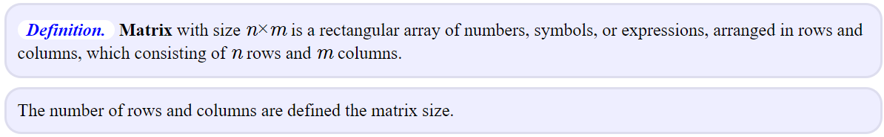
\includegraphics[height=6cm,width=1\textwidth,keepaspectratio]{matrix_def.png}
        % \caption{caption_name}
        \label{fig:matrix_def.png}
    \end{figure}
\end{frame}

\begin{frame}[t]{Operations with matrices}
\framesubtitle{}
\begin{columns}[T,onlytextwidth]
    \begin{column}{0.45\textwidth}
        \begin{exampleblock}{Between 2 or more matrices}
            \begin{itemize}
                \item Summation
                \item Multiplication (Order is important!)
                \item Cross Product
                \item Dot Product
            \end{itemize}
        \end{exampleblock}
        \alert{\textbf{\Large No Division!}}
    \end{column}
    \begin{column}{0.45\textwidth}
        \begin{exampleblock}{With one matrix}
            \begin{itemize}
                \item Multiplication on Scalar
                \item Length
                \item Transpose
                \item Trace
                \item Determinant
                \item Inverse Matrix
            \end{itemize}
        \end{exampleblock}
    \end{column}
\end{columns}

\end{frame}

\begin{frame}[t]{Summation and multiplication}
\framesubtitle{Case Study}
    \begin{figure}[H]
        \centering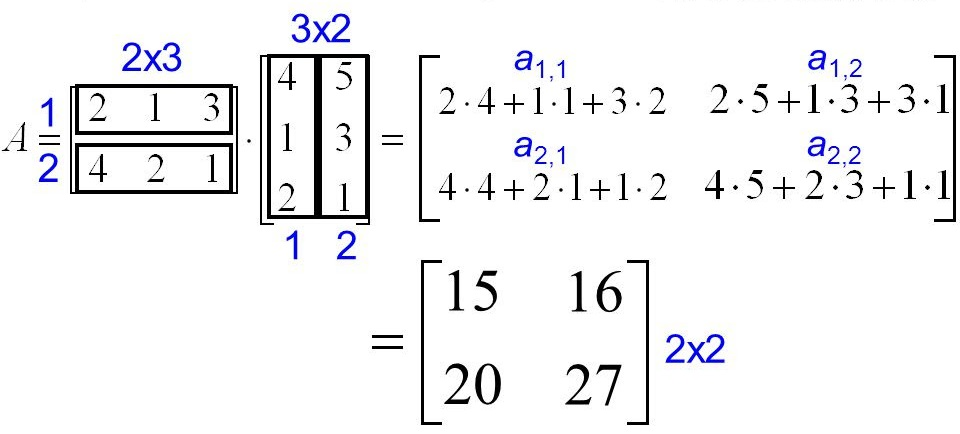
\includegraphics[height=5cm,width=1\textwidth,keepaspectratio]{matrix_multi_case.jpg}
        % \caption{caption_name}
        \label{fig:matrix_multi_case.jpg}
    \end{figure}
\end{frame}

\begin{frame}[t]{Transpose}
\framesubtitle{Case Study}
\begin{figure}[H]
    \centering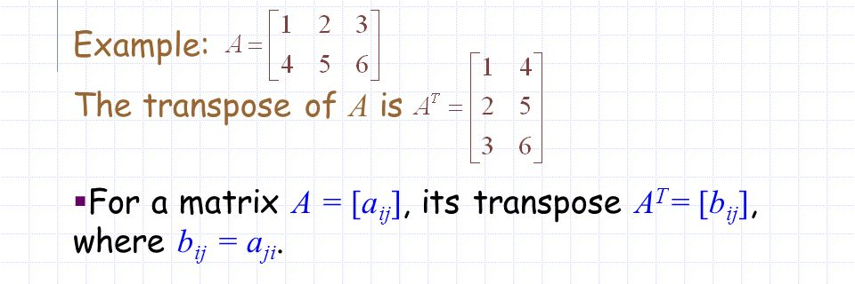
\includegraphics[height=5cm,width=1\textwidth,keepaspectratio]{transpose_case.png}
    % \caption{caption_name}
    \label{fig:transpose_case.png}
\end{figure} 
\end{frame}

\begin{frame}[t]{Transpose}
\framesubtitle{Why do we need it?}
    \begin{figure}[H]
        \centering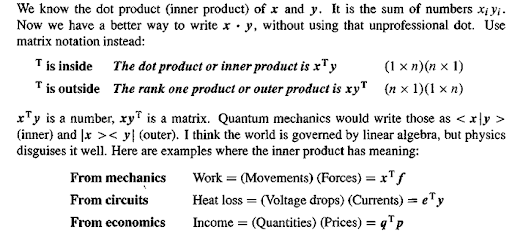
\includegraphics[height=5cm,width=1\textwidth,keepaspectratio]{transpose.png}
        % \caption{caption_name}
        \label{fig:transpose.png}
    \end{figure}
\end{frame}

\begin{frame}[t]{Trace}
\framesubtitle{Definition and Case Study}
\vspace{-0.3cm}
\begin{exampleblock}{Definition}
    The trace of an $n \times n$ square matrix $A$ is defined as:

    $\operatorname {tr} (\mathbf {A} )=\sum _{i=1}^{n}a_{ii}=a_{11}+a_{22}+\dots +a_{nn}$, where $a_{ii}$ denotes the entry on the $i$th row and $i$th column of $A$.\\  \textit{The trace is not defined for non-square matrices}.
\end{exampleblock}
$\mathbf {A} ={\begin{pmatrix}a_{11}&a_{12}&a_{13}\\a_{21}&a_{22}&a_{23}\\a_{31}&a_{32}&a_{33}\end{pmatrix}}={\begin{pmatrix}1&0&3\\11&5&2\\6&12&-5\end{pmatrix}}$
Then 
\begin{equation*}
    \operatorname {tr} (\mathbf {A} )=\sum _{i=1}^{3}a_{ii}=a_{11}+a_{22}+a_{33}=1+5+(-5)=1
    \phantom{\hspace{6cm}}
\end{equation*}
\end{frame}

\begin{frame}[t]{Intro to matrices}
    \framesubtitle{Task 1}
    Let $A=\begin{bmatrix} 3 & 1 \\ 5 & -2 \\ \end{bmatrix}$, $B=\begin{bmatrix} -2 & 1 \\ 3 & 4 \\ \end{bmatrix}$, $I=\begin{bmatrix} 1 & 0 \\ 0 & 1 \\ \end{bmatrix}$:
\begin{enumerate}
    \item Find $A+B$;
    \item Find $2A-3B+I$;
    \item Find $AB$ and $BA$ (make sure that, in general, $AB \neq BA$ for matrices);
    \item Find $AI$ and $IA$.
\end{enumerate}
\end{frame}

\begin{frame}[t]{Intro to matrices}
\framesubtitle{Task 2}
Let $A=\begin{bmatrix} 2 & -1 & -1\end{bmatrix}$ and $B=\begin{bmatrix} -2 \\ -1 \\ 3 \end{bmatrix}$:
\begin{enumerate}
    \item Find $AB$ and $BA$ if they exist;
    \item Find $A^TB$ and $BA^T$ if they exist.
\end{enumerate}   
\end{frame}

\begin{frame}[t]{Intro to matrices}
\framesubtitle{Task 3}
If solution exists, what the dimension of the result matrix. \\ There are several matrices: $\underset{3\times3}{A}$, $\underset{2\times3}{B}$, $\underset{3\times2}{C}$, $\underset{3\times5}{D}$, $\underset{3\times5}{D}$, $\underset{1\times2}{E}$, $\underset{3\times1}{K}$.
\begin{enumerate}
    \item $ABC$;
    \item $AB^TC^T$;
    \item $EBAE$;
    \item $AK \times K K^T B^T$.
\end{enumerate}
\end{frame}

\begin{frame}[t]{}
    % \vspace{-0.6cm}
    \begin{figure}[H]
        \centering
\includegraphics[height=7cm,width=1\textwidth,keepaspectratio]{english_meme.png}
        % \caption{caption_name}
        \label{fig:english_meme.png}
    \end{figure}
\end{frame}

\begin{frame}[t]{Determinant}
    \framesubtitle{Video}
    \vspace{-0.6cm}
    \begin{figure}[H]
        \href{https://youtu.be/Ip3X9LOh2dk}{
            \centering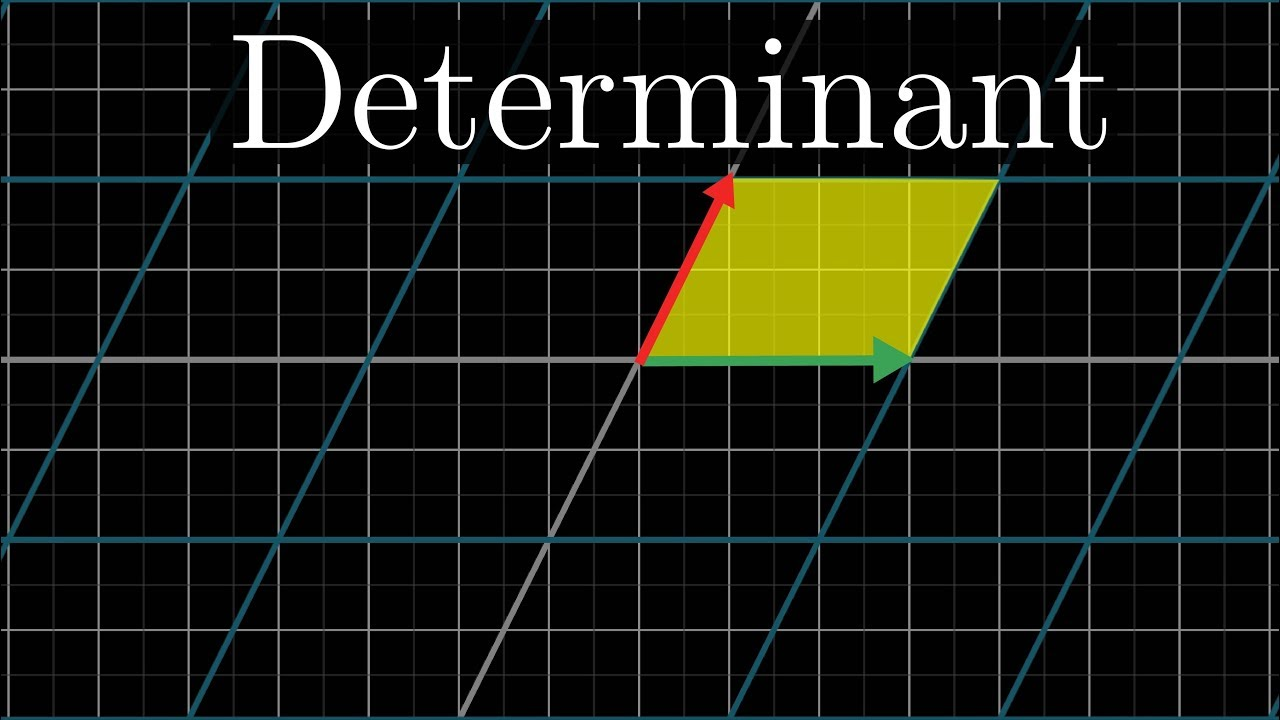
\includegraphics[height=6cm,width=1\textwidth,keepaspectratio]{det_brown.jpg}}
        % \caption{Click on a picture for a video}
        \label{fig:det_brown.jpg}
    \end{figure}
\end{frame}

\begin{frame}[t]{Determinant}
\framesubtitle{Where it can be used}
    \begin{enumerate}
        \item Find inverse matrix (next class)
        \item Find matrix rank (next class)
        \item Solve SLE using Cramer's rule (this HW)
    \end{enumerate}
\end{frame}

\begin{frame}[t]{Determinant}
\framesubtitle{How to Find (1)}
\vspace{-0.8cm}
\begin{equation*}
    \det(A)=\sum _{j=1}^{n}(-1)^{i+j}a_{ij}M_{ij}
    \phantom{\hspace{20cm}}
\end{equation*} \smallskip

The minor $M_{i,j}$ is defined to be the determinant of the $(n-1)\times (n-1)$-matrix that results from $A$ by removing the $i$-th row and the $j$-th column. \smallskip

\begin{equation*}
    \left\lvert \begin{matrix}
        a_{11} & a_{12} & a_{13} \\
        a_{21} & a_{22} & a_{23} \\ 
        a_{31} &  a_{32} & a_{33} 
        \end{matrix}\right\rvert = a_{11}\left\lvert \begin{matrix}
            a_{22} & a_{23} \\ 
            a_{32} & a_{33} 
        \end{matrix} \right\rvert  - a_{12}\left\lvert \begin{matrix}
            a_{21} & a_{23}\\ 
            a_{31}&  a_{33}
        \end{matrix} \right\rvert  + a_{13}\left\lvert \begin{matrix}
            a_{21} & a_{22} \\ 
            a_{31} &  a_{32}  
        \end{matrix} \right\rvert \phantom{\hspace{8cm}}
\end{equation*}
\end{frame}

\begin{frame}[t]{Determinant}
\framesubtitle{How to Find (2)}
\vspace{-0.5cm}
\begin{figure}[H]
    \centering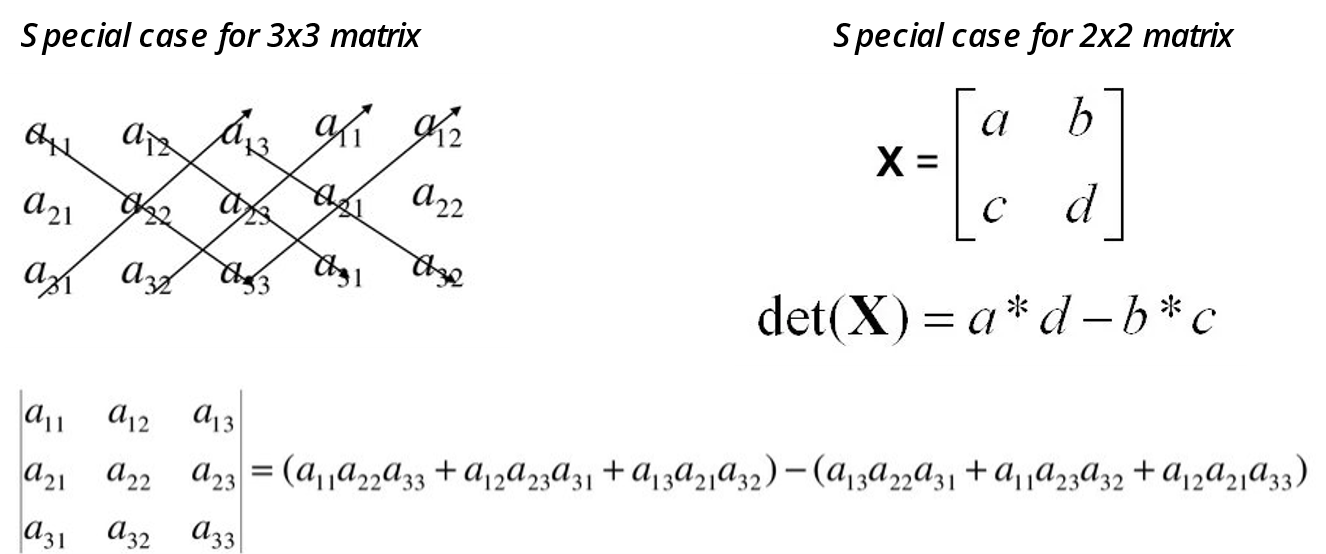
\includegraphics[height=5.5cm,width=1\textwidth,keepaspectratio]{detdet.png}
    % \caption{caption_name}
    \label{fig:detdet.png}
\end{figure}
\end{frame}

\begin{frame}[t]{Determinant}
\framesubtitle{Task 1}
Find the determinants of the following matrices:

(a) $A=\begin{bmatrix}
          5 & -2 \\
          1 & 6 \\
        \end{bmatrix}$;
(b) $B=\begin{bmatrix}
           1 & -3 & -1 \\
           -2 & 7 & 2 \\
           3 & 2 & -4 \\
         \end{bmatrix}$,
(c) $C=\begin{bmatrix}
    1 & -3 & -1 \\
    -2 & 0 & 2 \\
    3 & 0 & -4 \\
  \end{bmatrix}$
\end{frame}

\begin{frame}[t]{Determinant}
\framesubtitle{Task 2}
Find the matrix product $AB$ if $A=\begin{bmatrix}
    1 & 2 & 5 \\
    3 & 7 & x \\
  \end{bmatrix}$, $B=\begin{bmatrix}
     5 & -1 \\
     x & 2 \\
     -3 & -1 \\
   \end{bmatrix}$.\\ Then find the largest possible value of $det(AB)$.
\end{frame}

\begin{frame}[t]{}
    \framesubtitle{}
    % \vspace{-0.1cm}
    \begin{figure}[H]
        \begin{subfigure}{0.59\textwidth}
            \centering
\includegraphics[height=7cm,width=1\textwidth,keepaspectratio]{wolf1.png}
            % \caption{capture1}
            \label{fig:wolf1.png}
        \end{subfigure}
        \begin{subfigure}{0.39\textwidth}
            \centering
\includegraphics[height=7cm,width=1\textwidth,keepaspectratio]{wolf2.png}
            % \caption{capture2}
            \label{fig:wolf2.png}
        \end{subfigure}
    
    % \caption{capture_main}
    % \label{fig:}
    \end{figure}
\end{frame}

\begin{frame}[t]{Wolf Ballet}
    \framesubtitle{Video}
    \vspace{-0.6cm}
    \begin{figure}[H]
        \href{https://youtu.be/6krfziMgucI}{
            \centering
\includegraphics[height=6cm,width=1\textwidth,keepaspectratio]{wolf_video.jpg}}
        % \caption{Click on a picture for a video}
        \label{fig:wolf_video.jpg}
    \end{figure}
\end{frame}

\begin{frame}[t]{Scalar Triple Product}
\framesubtitle{Definition}
    \begin{columns}[T,onlytextwidth]
        \begin{column}{0.65\textwidth}
            $(a,b,c)$ --- is defined as the dot product of one of the vectors with the cross product of the other two. \bigskip

            \textbf{Geometrically} --- a signed volume of the parallelepiped defined by the three vectors given
              
        \end{column}
        \begin{column}{0.38\textwidth}
            \begin{figure}[H]
                \centering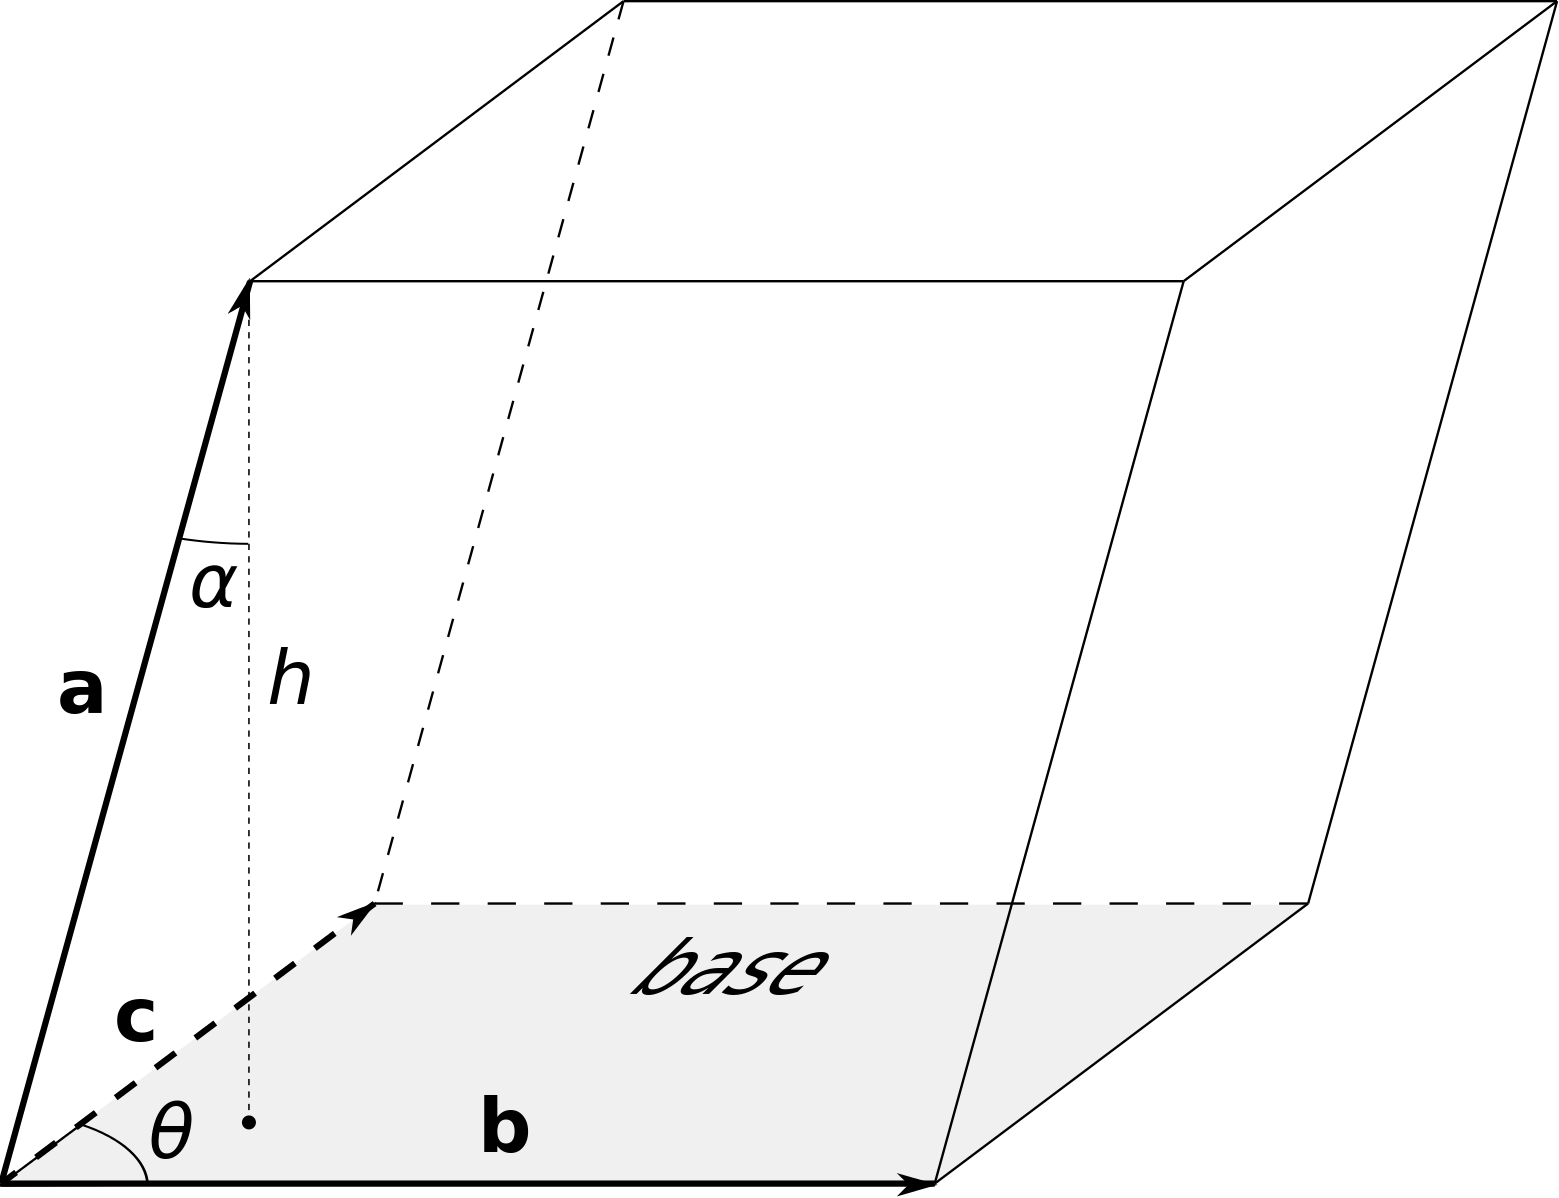
\includegraphics[height=6cm,width=1\textwidth,keepaspectratio]{scalar_triple.png}
                % \caption{caption_name}
                \label{fig:scalar_triple.png}
            \end{figure}
        \end{column}
    \end{columns}
\end{frame}

\begin{frame}[c]{Scalar Triple Product}
\framesubtitle{How to calculate}
\Large
    \begin{equation*}
        a \cdot (b \times c) = det(a,b,c) = det(\begin{bmatrix}
        a_1 & a_2 & a_3 \\
        b_1 & b_2 & b_3 \\ 
        c_1 & c_2  & c_3 
        \end{bmatrix})
    \end{equation*}
\end{frame}

\begin{frame}[t]{Scalar Triple Product}
\framesubtitle{Case Study}
    Calcute a triple scalar prodict between $\vec{a}$, $\vec{b}$ and $\vec{c}$.

    $\vec{a} = \begin{bmatrix}-1\\-1\\5\end{bmatrix},\ \vec{b} = \begin{bmatrix}1\\-1\\-2\end{bmatrix},\ \vec{c} = \begin{bmatrix}0\\-2\\3\end{bmatrix}$

    \begin{figure}[H]
        \centering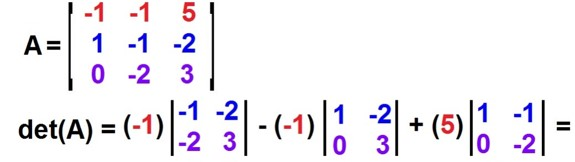
\includegraphics[height=3cm,width=1\textwidth,keepaspectratio]{triple_scalar_way.jpg}
        % \caption{caption_name}
        \label{fig:triple_scalar_way.jpg}
    \end{figure}
\end{frame}

\begin{frame}[t]{Scalar Triple Product}
\framesubtitle{Properties}
\vspace{-0.8cm}
    \begin{figure}[H]
        \centering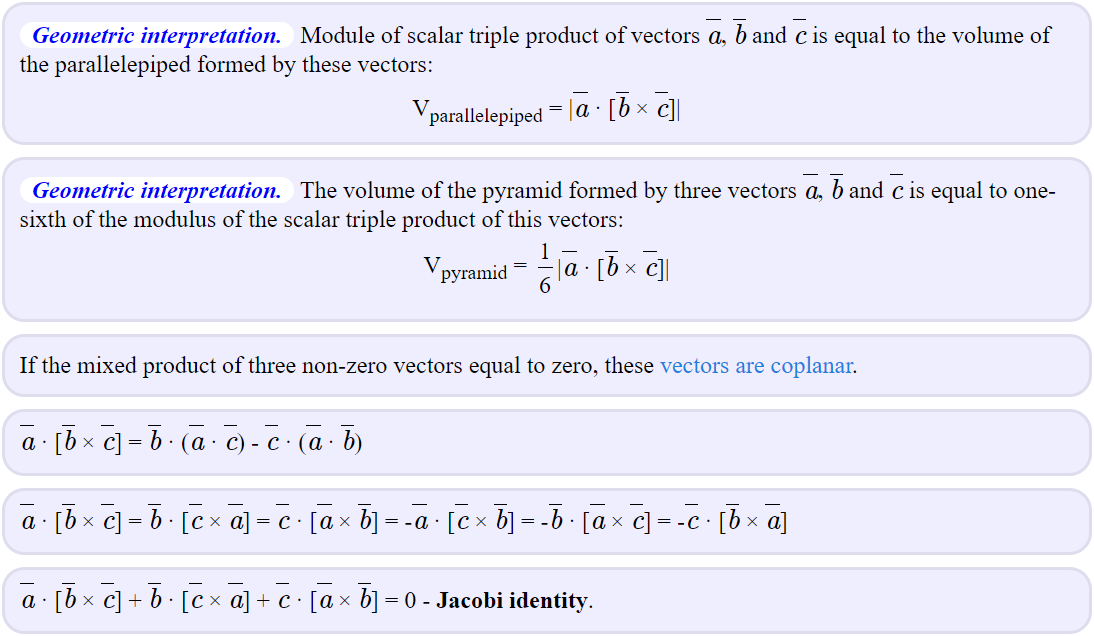
\includegraphics[height=6.2cm,width=1\textwidth,keepaspectratio]{triple_scalar_properites.png}
        % \caption{caption_name}
        \label{fig:triple_scalar_properites.png}
    \end{figure}
\end{frame}

\begin{frame}[t]{Scalar Triple Product}
\framesubtitle{Task 1}
Find the scalar triple product of $\textbf{a}=\begin{bmatrix} 1 \\ 2 \\ -1  \end{bmatrix}$, $\textbf{b}=\begin{bmatrix} 7 \\ 3 \\ -5  \end{bmatrix}$, $\textbf{c}=\begin{bmatrix} 3 \\ 4 \\ -3  \end{bmatrix}$.
\end{frame}

% \begin{frame}[t]{Scalar Triple Product}
% \framesubtitle{Task 2}
% Vectors $\textbf{a}$, $\textbf{b}$, $\textbf{c}$ are not coplanar. Find all values of $\theta$ such that vectors $\textbf{a}+2\textbf{b}+\theta\textbf{c}$, $4\textbf{a}+5\textbf{b}+6\textbf{c}$, $7\textbf{a}+8\textbf{b}+\theta^2\textbf{c}$ are coplanar.
% \end{frame}

\begin{frame}[t]{Reference material}
    \framesubtitle{OnlineMschool}
    \Large
    \begin{itemize}
        \item \href{https://onlinemschool.com/math/library/matrix/definition/}{Matrix definition}
        \item \href{https://onlinemschool.com/math/library/matrix/multiply/}{Matrix multiplication}
        \item \href{https://onlinemschool.com/math/library/matrix/transpose/}{Transpose}
        \item \href{https://onlinemschool.com/math/library/matrix/determinant/}{Determinant}
        \item \href{https://onlinemschool.com/math/library/vector/multiply2/}{Scalar Triple Product}
    \end{itemize}
\end{frame}

\fbckg{fibeamer/figs/last_page.png}
\frame[plain]{}

\end{document}